\section{$k$-Tree and graph scan statistics}
\label{sec:applications}
We now describe how \ouralgo{} for the $k$-path problem can be extended to 
parallel algorithms for finding trees and optimizing scan statistics. We discuss here how the corresponding polynomials are constructed recursively and evaluated in the subroutines \parcircuittree{} and \parcircuitscan{};
the main Algorithm \ouralgo{} remains unchanged.

\subsection{$k$-Tree}
\label{sec:apps-trees}
\begin{figure}[h]
\vspace{-0.2in}
\centering
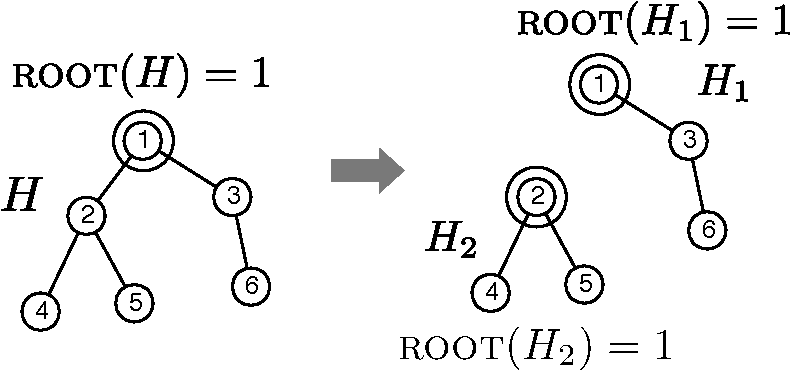
\includegraphics[width=0.37\textwidth]{img/trees.pdf}
\caption{
\small
Tree $H$ with $\myroot(H)=1$ is decomposed into trees $H_1$ and $H_2$ by
removing edge $(1, 2)$: $\myroot(H_1)=1$ and $\myroot(H_2)=2$.
%\vspace{-0.2in}
}
\label{fig:trees}
\end{figure}
We describe how an instance of $k$-Tree with graph $G=(V,E)$ and tree $H=(V^H, E^H)$
is reduced to a $k$-MLD instance. We consider the tree $H$ to be rooted,
and let $\myroot(H)$ be the root node, selected arbitrarily. We consider a hierarchical
structure among subtrees of $H$ in the following manner: consider any node $u\in\nbr(\myroot(H))$.
Let $H_1$ and $H_2$ denote the subtrees or \emph{children} obtained upon deleting the edge $(u, \myroot(H))$,
with $\myroot(H)\in H_1$ and $u\in H_2$. We set $\myroot(H_1)=\myroot(H)$ and $\myroot(H_2)=u$.
This process is illustrated in Figure \ref{fig:trees}.
The subtrees $H_1$ and $H_2$ are further partitioned in a recursive manner until
all trees have a single node.
We define the polynomials $P(i, H')$, which will correspond to all layouts (not necessarily
isomorphisms) of $H'$ with $\myroot(H')=i$ for all nodes $i \in V$, as follows:
\begin{itemize}
\item
If $H'$ consists of a single node, $P(i, H') = x_i$
\item
Else, 
$P(i, H') = \sum_{u\in\nbr(i)} P(i, H'_1)P(u, H'_2)$, where
$H'_1$ and $H'_2$ are the children of $H'$.
\item
Finally, we have
$P(x_1,\ldots, x_n)= \sum_{i \in V} P(i, H)$
\end{itemize}

By using ideas from \cite{alon2008biomolecular}, it can be verified that the tree $H$ is a subgraph of $G$ if and only if the
polynomial $P(x_1,\ldots,x_n)$ has a multilinear term. Algorithm \parcircuittree{}
evaluates this polynomial analogous to Algorithm \ref{alg:parEvaluatepath} from Section \ref{sec:proposed}. The performance of \ouralgo{} using \parcircuittree{} is summarized below.

\begin{lemma}
\label{lemma:parmaxwt-tree}
For any $\epsilon\in(0, 1)$,
Algorithm \ouralgo{}, using \parcircuittree{}, solves the \textsc{$k$-Tree} problem for an
instance $(G, H)$ with probability at least $1-\epsilon$. The total time for
computation and communication are $O\left(c_1\frac{2^kN_1}{N}|\mathcal{T}| \maxload{}\log{1/\epsilon}\right)$ 
and $O\left(c_2\frac{2^kN_1}{N N_2}|\mathcal{T}| \maxdeg{}\log{1/\epsilon}\right)$, respectively.
\end{lemma}

\begin{algorithm}{}
\small
\caption{\parcircuittree{$(G(V, E), H(V^H, E^H), \mathbf{v}, t, N_2, N_1, \mathcal{P})$}}
\label{alg:parEvaluatepath} 
\begin{algorithmic}[1]
\STATE \textbf{Input:} Graph $G(V, E)$, tree $H(V^H, E^H)$ with $k$ vertices, 
random assignment $\mathbf{v}$, phase number $t$, number of iterations within phase $N_2$,
number of partitions $N_1$, and partitioning $\mathcal{P}$
\STATE \textbf{Output:} The value of the polynomial corresponding to $k$-tree in the iterations within a phase
\STATE
\STATE Let $\mathcal{T}$ be a collection of subtrees of $H$ sorted by size
\STATE \textbf{for} each processor $s$\textbf{do in parallel}
\STATE \quad \textbf{for} each subtree $j \in \mathcal{T}$ \textbf{do}
\STATE \quad \quad \textbf{for} node $i\in G^s$ and iteration $q\in [tN_2,(t+1)N_2 - 1]$ \textbf{do}
\STATE \quad \quad \quad \textbf{if} $|j|=1$ \textbf{then}
\STATE \quad \quad \quad \quad $P(i, q, j) = 1 + (-1)^{v_i^T \cdot q_{\text{bin}}}$
\STATE \quad \quad \quad \textbf{else}
\STATE \quad \quad \quad \quad set $P(i,q, j) = 0$
\STATE \quad \quad \quad \quad let $j'$ and $j''$ be the children of subtree $j$
\STATE \quad \quad \quad \quad \quad \textbf{for} each incoming message $\langle u, P(u, q, j'')\rangle$ \textbf{do}
\STATE \quad \quad \quad \quad \quad \quad $P(i, q, j)= P(i, q, j) + P(i, q, j')  P(u, q, j'')$
\STATE \quad \quad \quad \textbf{Send result to neighbors}
\STATE \quad \quad \quad  \textbf{for} $u \in \nbr(i)\setminus G^s$ \textbf{do}
\STATE \quad \quad \quad \quad \textbf{Send} $\langle i, P(i, q, j)\rangle$
\STATE \textsc{MpiBarrier}
\STATE \textbf{return} $\sum_q \sum_i P(i, q, H)$
\end{algorithmic}
\end{algorithm}

More generally, we consider a weighted version of the problem, where the goal is to find an embedding of the maximum weight. We also note that the algorithm can be generalized to find motifs of bounded treewidth, similar to algorithms based on the color coding technique. \cite{alon1995color}.

\iffalse
\comment{move the rest of this to the supplementary}

\begin{figure}[h]
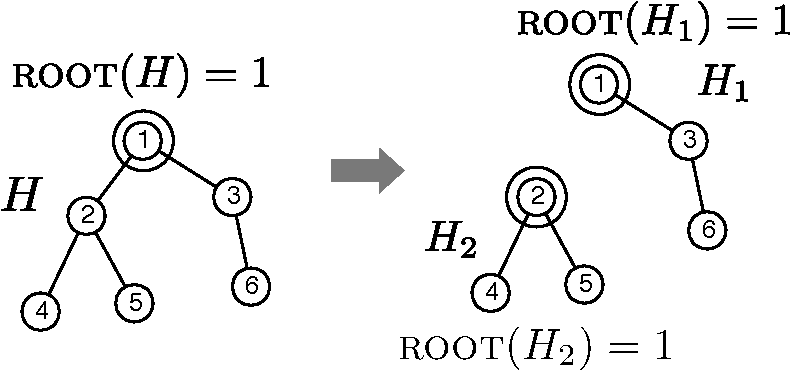
\includegraphics[width=0.4\textwidth]{img/trees.pdf}
\caption{
\small
Tree $H$ with $\myroot(H)=1$. It is decomposed into trees $H_1$ and $H_2$ by
removing the edge $(1, 2)$. $\myroot(H_1)=1$ and $\myroot(H_2)=2$.
%\vspace{-0.2in}
}
\label{fig:trees}
\end{figure}
Next, we consider the case where $H$ is a tree. We consider the tree to be rooted,
and let $\myroot(H)$ be the root node, selected arbitrarily. We consider a hierarchical
structure among subtrees of $H$ in the following manner: consider any node $u\in\nbr(\myroot(H))$.
Let $H_1$ and $H_2$ denote the subtrees obtained upon deleting the edge $(u, \myroot(H))$,
with $\myroot(H)\in H_1$ and $u\in H_2$. We set $\myroot(H_1)=\myroot(H)$ and $\myroot(H_2)=u$.
This process is illustrated i Figure \ref{fig:trees}.
The subtrees $H_1$ and $H_2$ are further partitioned in a recursive manner, till
all trees have a single node. For an intermediate tree $H'$ in this process,
let $\textsc{child}_1(H')$ and $\textsc{child}_2(H')$ denote the two child trees
resulting from the tree $H'$. Let $\textsc{parent}(H')=H''$ be the tree such that
either $\textsc{child}_1(H'')= H'$ or $\textsc{child}_2(H'') = H'$.
We define the polynomials $P_v(H')$, which will correspond to all layouts (not necessarily
isomorphisms) of $H'$ with $\myroot(H')=v$, in the following manner:
\begin{itemize}
\item
If $H'$ consists of a single node, $P_v(H') = x_v$
\item
Else, 
$P_v(H') = \sum_{u\in\nbr(v)} P_v(H'_1)P_u(H'_2)$, where
$H'_1$ and $H'_2$ denote $\textsc{child}_1(H')$ and $\textsc{child}_2(H')$, respectively.
\item
Finally, we have
$P(x_1,\ldots, x_n)= \sum_v P_v(H)$
\end{itemize}

More generally, we consider a weighted version of the problem, where the goal is to find an embedding of the maximum weight. We also note that the algorithm can be generalized to find motifs of bounded treewidth similar to algorithms based on the color coding technique. \cite{alon1995color}.
\fi 

\subsection{Scan Statistics}
\label{sec:apps-scanstat}
%For concreteness, we now show how to implement a sequential algorithm for Problem \ref{prob:macs} based on the Multilinear Detection technique. We start by describing how to recursively construct and evaluate a circuit for this problem.
Let $W(V) = \sum_{i\in V}{w(i)}$ be the total weight of the nodes in $G$. For each node $i$, we define a variable $x_i$, and we construct a polynomial over the set of variables $\{x_i: i \in V\}$. Every term---i.e., monomial---in this polynomial will represent a connected subgraph of size at most $k$ and weight at most $W(V)$.
For $j \leq k$ and $z \leq W(V)$, let $P(i,j,z)$ be the polynomial corresponding to a subgraph (1) containing node $i$, (2) of size $j$, and (3) total weight $z$. The following recurrence relations describe how the polynomials $P(i, j, z)$ are computed:
\begin{itemize}
\item
$P(i, 1, z) = x_i$ for all $i \in V$, $z = w(v)$
\item
For $i \in V$, $j = 2$ to $k$, $z = 0$ to $W(V)$, 
$P(i,j, z) = \sum_{u \in \nbr(i)} \sum_{j' = 1}^{j-1}\sum_{z'=0}^z (P(i, j', z') \cdot P(u, j - j', z-z'))$
\item
$P(j, z) = \sum_i P(i,j, z)$ for $j \leq k$, $z \leq W(V)$
\end{itemize}
Algorithm \ref{alg:parEvaluateScanStat} maintains variables $P(i, q, j, z)$ for every node $i$, $j\leq k$, $z \leq W(V)$, and iteration $q$ within phase $t$. It can be verified \cite{cadena:bigdata17} that the input graph $G$ has a connected subgraph $S$ of size $j$ and weight $z$ if and only if the corresponding polynomial $P(j, z)$ has a multilinear term.
We have the following lemma.
%The performance of \ouralgo{}, using \parcircuittree{} is summarized below.

\begin{lemma}
\label{lemma:parmaxwt-scan}
For any $\epsilon\in(0, 1)$,
Algorithm \ouralgo{}, using \parcircuitscan{}, solves the \textsc{Scan Statistics} problem for an
instance $(G, k, \mathbf{w})$, with probability at least $1-\epsilon$. The total time for
computation and communication are $O\left(c_1\frac{2^kN_1}{N}W(V)^2k^2 \maxload{}\log{1/\epsilon}\right)$ 
and $O\left(c_2\frac{2^kN_1}{N N_2}W(V)^2k^2 \maxdeg{}\log{1/\epsilon}\right)$, respectively.
\end{lemma}

We note that the performance for scan statistics can be improved significantly by rounding the weights, using a standard technique as in the Knapsack problem \cite{cadena:bigdata17}.

%\noindent
%\subsubsection{High level idea of \textsc{MLD-ScanStat} (Algorithm \ref{alg:mld-scanstat})}
%After selecting random vectors from $\mathbb{Z}_2^k$ for each circuit input (line 6), 
%we compute the polynomial by performing $2^k$ evaluations of the circuit (lines 8--24). 
%The $t$-{th} evaluation gives us the value of the $(t + 1)$-th row in the matrix 
%representation, as discussed in Section \ref{sec:prelim}. We evaluate the circuit following its recursive definition. First, we initialize the circuit inputs in the base case (lines 11--13) 
%to be the $t$-th eigenvalue of their respective matrix representation, which is computed 
%as $1 + (-1)^{x_v^T\cdot t_{\text{bin}}}$, where $x_v$ is the random vector assigned to node 
%$i$ and $t_{\text{bin}}$ is the $k$-bit binary representation of $t$. 
%Then, for each $i \leq k$, we evaluate the circuit by aggregating values from nodes of the form $P_v(i')$, for some $i' < i$, which have already been computed in 
%a previous iteration of the \textbf{for} loop. 
%We show an example of this algorithm in Figure \ref{fig:algorithm-example}.

%%%\begin{figure*}[!htbp]
%%%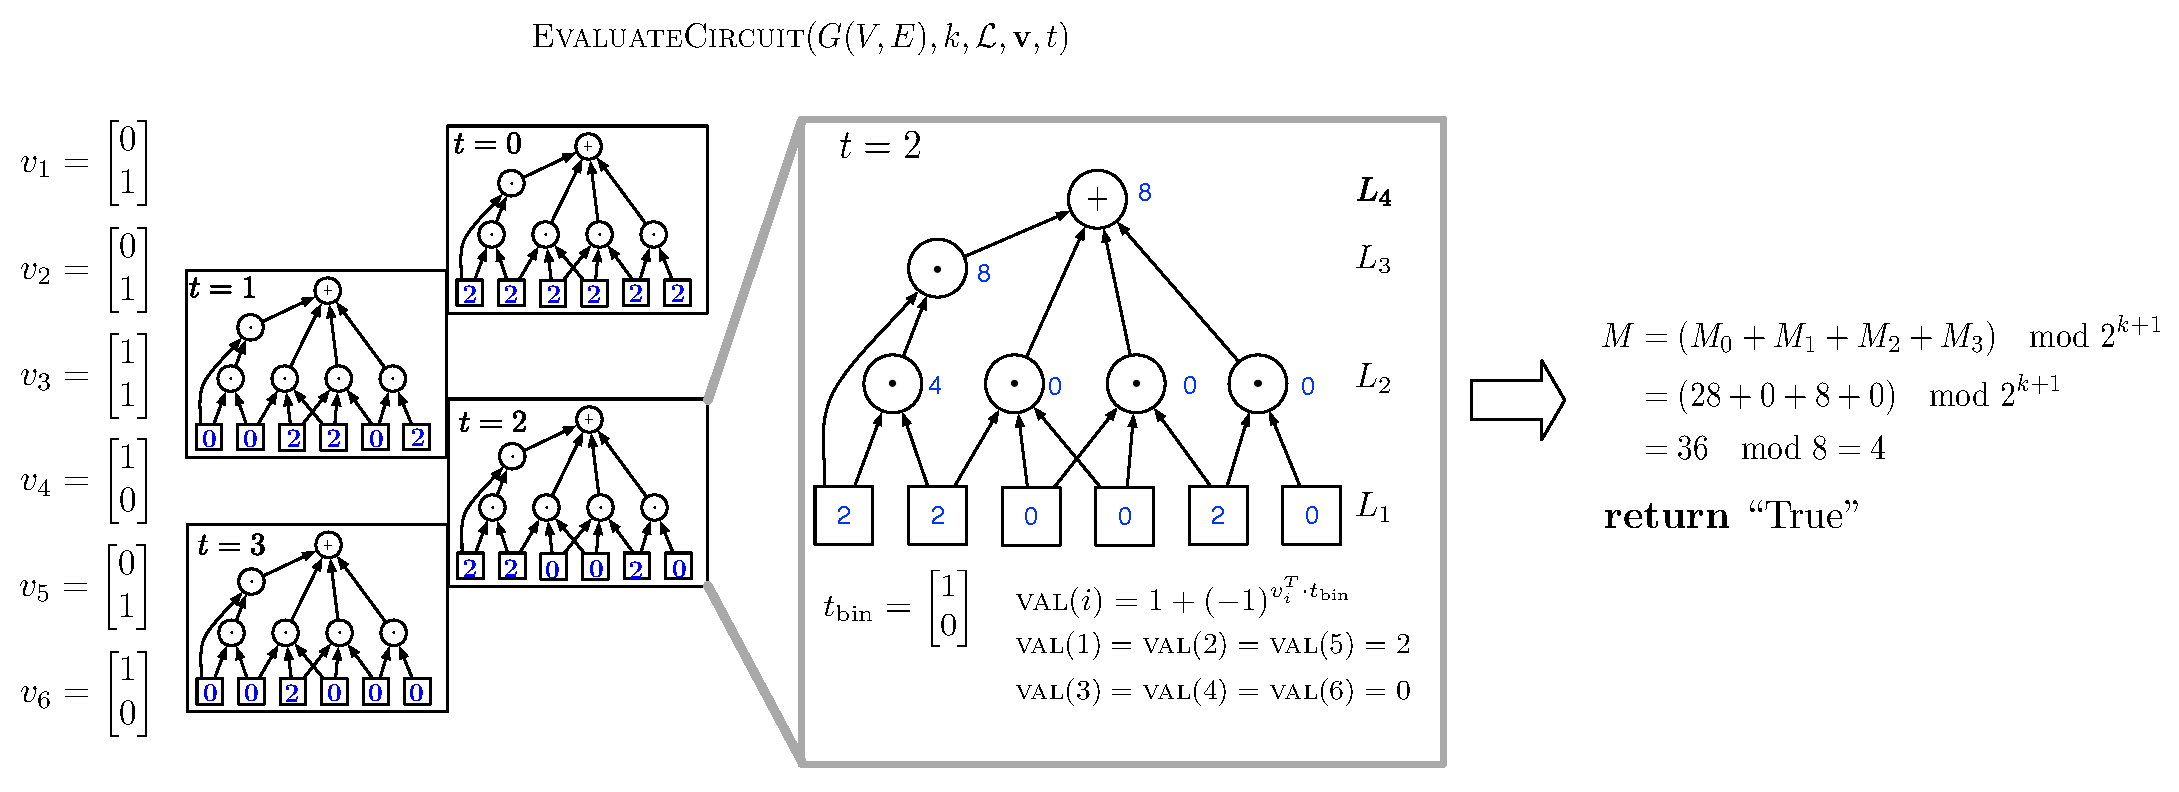
\includegraphics[width=\textwidth]{img/algorithm-example-v2_fixed.pdf}
%%%\caption{
%%%\small
%%%Example of the sequential algorithm \maxwt{}. The input is the circuit $G(V,E)$ from
%%%Figure \ref{fig:dag} with 12 nodes on four levels, $L_1$, $L_2$, $L_3$ and $L_4$, as shown.
%%%The algorithm picks the vectors $v_1,\ldots,v_6$ from $\mathbb{Z}_2^2$, as shown in
%%%the left of the figure. Since $k=2$, there are $2^k=4$ iterations, corresponding to
%%%$t=0,\ldots,3$. The values of $\val(v)=1+(-1)^{v^Tt_{bin}}$ for the $t$th iteration
%%%are shown in blue as the input values. The outputs of the circuit are $M_0, \ldots, M_3$,
%%%with values as shown in the right of the figure. For these choices of the $v_i$'s, the
%%%computed value $M\neq 0 (\text{mod } 2^{k+1})$, which implies the existence of a
%%%multilinear term with $k$ variables. This is true because the term $x_5x_6$ in the
%%%polynomial is indeed multilinear.
%%%%---IDs are in red---$k=2$, and 3 levels. Nodes 1 through 6 are the first level---i.e., the circuit inputs. Nodes 7 through 10 are the second level, all with multiplication operation ($op(i) = \cdot$). The last level only contains the root of the circuit, with addition operation. First, the algorithm generates random vectors $v_i$ for the circuit inputs (bottom left). Then, the circuit is evaluated $2^k$ times by calling procedure \algcircuit{} (center). We show the evaluation for iteration $t=2$. First, we compute the inputs to the circuit as $1 + (-1)^{v_i^T\cdot t_{\text{bin}}}$---this will always be either 2 or 0. From there, we can evaluate the circuit by levels. Finally, back in \maxwt{}, we aggregate the value at root$(G)$ over all the iterations (right). In this case, the polynomial evaluates to $0$, so we return ``False".
%%%%\vspace{-0.2in}
%%%}
%%%\label{fig:algorithm-example}
%%%\end{figure*}

%\begin{algorithm}{}
%\small
%\caption{\maxwt{}$(G(V, E), k$.}
%\label{alg:multilinear-detect}
%\begin{algorithmic}[1]
%\STATE \textbf{Input}: Graph $G(V, E)$, parameter $k$
%\STATE\textbf{Output}: ``True" if circuit evaluation is non-zero. ``False" otherwise.
%\STATE \textbf{Initialize circuit inputs}
%\STATE \textbf{for} node $i \in L_1$ \textbf{do}
%\STATE \quad Let $v_i$ be a random vector from $\mathbb{Z}_{2}^k$
%\STATE \textbf{Initialize the polynomial}
%\STATE Let $M = \bar 0$
%\STATE \textbf{Evaluate circuit for each row of matrix representation}
%\STATE \textbf{for} $t = 0$ to $2^{k-1}$ \textbf{do}
%\STATE \quad $M_t = \algcircuit(G(V, E), k, \mathcal{L}, \mathbf{v}, t)$
%\STATE $M = \sum_{t=0}^{2^{k-1}} M_t \mod 2^{k+1}$
%\STATE \textbf{return} $M \neq 0$
%\STATE
%\STATE \textbf{procedure} \algcircuit{$(G(V, E), k, \mathcal{L}, \mathbf{v}, t)$}
%\STATE \textbf{Input}: Circuit $G(V, E)$, parameter $k$, node levels $\mathcal{L}$, random assigment $\mathbf{v}$, and iteration number $t$
%\STATE\textbf{Output}: Value at root node of $G(V,E)$
%\STATE \textbf{Initialize circuit inputs}
%\STATE \textbf{for} node $i \in L_1$ \textbf{do}
%\STATE \quad $ \val(i) = 1 + (-1)^{v_i^T \cdot t_{\text{bin}}}$
%
%\STATE \textbf{Evaluate the circuit by levels}
%\STATE \textbf{for} $s=2$ to $|\mathcal{L}|$ \textbf{do}
%\STATE \quad \textbf{for} $i \in L_s$ \textbf{do}
%\STATE \qquad \textbf{if} $\op(i) = +$ \textbf{then}
%\STATE \qquad \quad $\val(i) = 0$
%\STATE \qquad \quad \textbf{for} $j \in \pred(i)$ \textbf{do}
%\STATE \qquad \qquad $\val(i) = \val(i) + \val(j)$
%\STATE \qquad \textbf{else} 
%\STATE \qquad \quad $\val(i) = 1$
%\STATE \qquad \quad \textbf{for} $j \in \pred(i)$ \textbf{do}
%\STATE \qquad \qquad $\val(i) = \val(i) \cdot \val(j)$
%
%\STATE \textbf{return} $\val($root$(G))$
%\end{algorithmic}
%\end{algorithm}

%\begin{algorithm}{}
%\small
%\caption{\small \textsc{MLD-ScanStat}$(G(V, E), \mathbf{w}, k, \epsilon, r)$.}
%\label{alg:mld-scanstat}
%\begin{algorithmic}[1]
%\STATE \textbf{Input}: Instance $(G(V, E), \mathbf{w})$ and parameters $k, \epsilon, r$
%\STATE\textbf{Output}: "True" if $G$ has a subgraph $S$ with size $i \leq k$ and weight $j \leq r$
%\STATE Let $K=\{1,\ldots,k\}, R=\{0, \ldots, r\}$
%\STATE \textbf{Initialize the polynomial}
%\STATE $P(i, j) = \bar{0}$ for $i \in K$, $j \in R$
%\STATE For each node $v$, pick a random vector $x_v \in Q[\mathbb{Z}_{2}^k]$
%\STATE \textbf{Evaluate the circuit for each row of matrix representation}
%\STATE \textbf{for} $t = 0$ to $2^{k-1}$
%\STATE \quad $P_v(i, j) = \bar{0}$ for $i \in K$, $j \in R$
%\STATE \quad \textbf{Initialize circuit inputs}
%\STATE \quad \textbf{for} $v \in V$ \textbf{do}
%\STATE \quad \quad $P_v(1, w(v)) = 1 + (-1)^{x_v^T \cdot t_{\text{bin}}}$
%\STATE \quad \textbf{Evaluate circuit recursively}
%\STATE \quad \textbf{for} $v \in V$, $i = 2$ to $k$, $j = 0$ to $r$ \textbf{do}
%\STATE \qquad $P_v(i,j) = \sum_{u \in \nbr(v)} \sum_{i' = 1}^{i-1}\sum_{j'=0}^j (P_v(i', j') \cdot P_u(i-i', j - j'))$ 
%\STATE
%\STATE \textbf{return} $P \neq \bar 0$
%\end{algorithmic}
%\end{algorithm}

\begin{algorithm}{}
\small
\caption{\parcircuitscan{$(G(V, E), k, \textbf{w}, \mathbf{v}, t, N_2, N_1, \mathcal{P})$}}
\label{alg:parEvaluateScanStat} 
\begin{algorithmic}[1]
\STATE \textbf{Input:} Graph $G(V, E)$, parameter $k$, node weights $\mathbf{w}$, 
random assignment $\mathbf{v}$, phase number $t$, number of iterations within phase $N_2$,
number of partitions $N_1$, and partitioning $\mathcal{P}$
\STATE \textbf{Output:} The value of the polynomial corresponding to the scan statistics in the iterations within a phase
\STATE
\STATE \textbf{for} each processor $s$ \textbf{do in parallel}
\STATE \quad \textbf{for} node $i \in G^s$ and iteration $q \in [tN_2,(t+1)N_2-1]$ \textbf{do}
\STATE \qquad $ P(i, q, 1, w(v)) = 1 + (-1)^{v_i^T \cdot q_{\text{bin}}}$
\STATE \quad \textbf{for} $j=2$ to $k$ and $z=0$ to $W(V)$ \textbf{do}
\STATE \qquad \textbf{for} node $i \in G^s$ \textbf{do}
\STATE \qquad \quad \textbf{for} all $q$ set $P(i,q, j, z) = 0$
\STATE \qquad \quad \textbf{for} each incoming message $\langle u, P(u, q, j-j', z-z')\rangle$ \textbf{do}
\STATE \qquad \qquad $P(i, q, j, z)= P(i, q, j, z) + P(i, q, j', z')  P(u, q, j-j', z-z')$
\STATE \qquad \quad  \textbf{Send result to neighbors}
\STATE \qquad \quad \textbf{for} $u \in \nbr(i)\setminus G^s$ \textbf{do}
\STATE \qquad \qquad \textbf{Send} $\langle i, P(i, q, j, z)\rangle$
\STATE \textsc{MpiBarrier}
\STATE \textbf{return} $\sum_q \sum_i P(i, q, k, z)$ for all $z \leq W(V)$
\end{algorithmic}
\end{algorithm}